\chapter{Performance regression using Gumby}

\section{Introduction to Gumby}
\begin{figure}[h]
	\makebox[\textwidth][c]{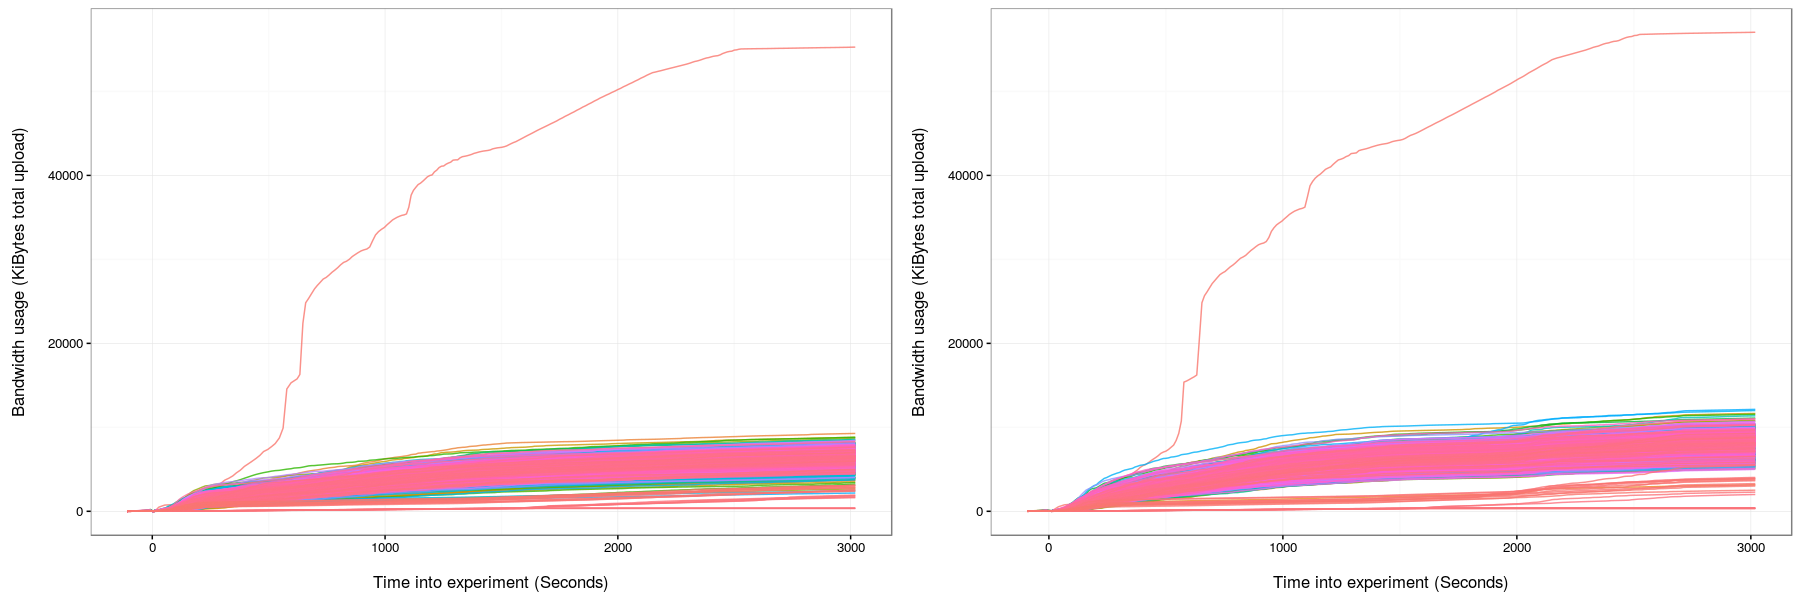
\includegraphics[width=\linewidth]{experimentation/images/send.png}}
	\caption{An example of a side by side comparison of two \enquote{allchannel} experiment runs. Left the current code base, right asynchronous Dispersy with blocking I/O.}
	\label{fig:side_by_side_send}
\end{figure} 

Tribler has an experiment runner framework for Dispersy and Tribler: Gumby.
Using Gumby, one can specify configurations and scenario files to be executed.

Configuration files specify all the settings needed in order to run an experiment using Gumby.
Scenario files allow for a carefully timed execution of functions; each line in a scenario file specifies which nodes execute which function at what time. \todo{Example of such a scenario file? yes/no?}
Currently, Gumby is being used to run an experiment on the DAS5 super computer\footnote{\url{http://www.cs.vu.nl/das5/}}.
Whenever a push happens on a pull request on GitHub, our Jenkins continuous integration system automatically schedules this experiment to be run.

Using Gumby, statistics such as CPU, memory consumption and I/O are automatically tracked.
Any additional information that one wishes to track can be logged and parsed using auxiliary post experiment scripts.
Currently, graphs are being generated in the R programming language using the ggplot2 library.

To realize a regression testing system, we decided to extend Gumby with additional functionalities and scripts.
First the proposed commits first have to be run inside an experiment using a predetermined scenario and configuration file.
This will produce data about the changes made to the codebase.
Once this experiment is done, Jenkins can fetch the performance data of the current code base, which we can compare against.
To create a comparison that requires little effort to interpret, graphs \todo{and tables?} will be generated.
By creating a side-by-side plot of two graphs using the same scales, developers can immediately see any changes, see Figure~\ref{fig:side_by_side_send}.\todo{Replace the right one with the dispersy async + non-block, should be more of a change.}

\section{Performance regression using Gumby}

\section{Continuous regression testing using Jenkins}


\section{Representative benchmarks}

We created representative benchmarks, good use cases of tribler etc.

\section{Multiple platforms}

windows 32 and 64 bit, osx, linux

\section{Validating the performance regression system}

To validate the performance regression system, we have resolved one of Tribler's biggest bottlenecks: Dispersy's blocking database I/O.
To address this problem, we have written Dispersy's I/O to become asynchronous and non-blocking.
To realize this, a new database manager \enquote{StormDBManager} is introduced and 90\%\todo{made up number, need to calculate the actual value.} of Dispersy's functions have been refactored.